\chapter{Análisis del problema y diseño de la solución}

Para este TFG se quiere conseguir una predicción en el mundo del fútbol para poder decir con cierta seguridad el ganador de un partido. Para ello, se ha diseñado un algoritmo que utiliza las estadísticas de los futbolistas, entre ellas su mapa de calor, para predecir el ganador, y después, respaldar ese resultado con una base de datos con los resultados de partidos ya jugados.

\section*{Definición del algoritmo}
Este algoritmo presenta un modelo analítico para predecir el resultado de un partido de fútbol, basado en las estadísticas individuales de los jugadores y de sus mapas de calor. Se separan las estadísticas en categorías constructivas y destructivas, se normalizan y se ponderan según la distribución espacial de cada jugador en el campo, dividiendo el campo en zonas con distintos pesos. El modelo evalúa la ventaja en cada zona mediante una simetría entre zonas ofensivas y defensivas, para finalmente construir un score final que permite definir el ganador del partido. Más adelante, mediante un algoritmo genético, se intentará optimizar los pesos que se le dan a cada zona para intentar obtener el máximo rendimiento posible.

\section{Base de datos}
En el ámbito del análisis deportivo, especialmente en el fútbol, resulta de gran interés predecir el resultado de un partido de fútbol a partir de datos complejos que van más allá del simple marcador. En este proyecto se parte de una base de datos de partidos de la liga española, tanto femenina como masculina, en la que se dispone de tres tipos de información:

\begin{itemize}
    \item Resultado del partido: se almacena quien gana, empata o pierde el partido, así como el local, visitante y la temporada en que se jugó.
    \item Mapas de calor de cada jugador: muestra la distribución espacial de su actividad en el partido.
    \item Estadísticas individuales de cada jugador en el partido: pueden ser constructivas o destructivas.
    
\end{itemize}

Para la implementación del sistema se ha optado por el uso de MongoDB como sistema de gestión de bases de datos no relacional debido a su flexibilidad y facilidad con el tratamiento de los datos. Aunque también se ha hecho uso de MongoDB Compass como interfaz gráfica, debido a que todo es mucho más intuitivo y fácil de mostrar.

Para el almacenamiento de los partidos ya jugados se han almacenado los atributos de local, visitante, temporada y el ganador del partido. No se ha visto necesario almacenar el número de goles, pues no nos interesa saber por cuánto se ha ganado el partido, sino quién lo ha ganado. La descripción de los atributos es la siguiente:

\begin{table}[H]
    \centering
    \begin{tabular}{|c|c|}
        \hline
        \textbf{Atributo} & \textbf{Descripción} \\
        \hline
        Local & Nombre del equipo que jugó el partido como local \\
        \hline
        Visitante & Nombre del equipo que jugó el partido como visitante \\
        \hline
        Temporada & Temporada en la que se jugó el partido \\
        \hline
        Resultado & Indica si la victoria fue local, visitante o hubo empate \\
        \hline
    \end{tabular}
    \caption{Atributos de los partidos de la base de datos}
    \label{tab:ejemplo}
\end{table}

También es importante aclarar que en el fútbol español, para diferenciar a los equipos masculinos y femeninos se les añade un 'F' al final del nombre, por lo que esta será la manera de almacenarlos en la base de datos y de diferenciarlos con los masculinos. Un ejemplo implementado desde MongoDB Compass sería:

\begin{figure}[H]
    \centering
    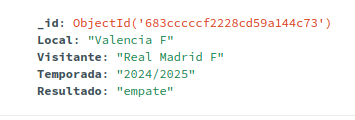
\includegraphics[width=0.7\textwidth]{plantilla-TFG-ETSIIT/doc/imagenes/BD_partido.png}
    \caption{Entrada de partido en MongoDB Compass}
    \label{fig:etiqueta-imagen}
\end{figure}

Después, para cada partido se almacenan las estadísticas individuales de cada futbolista de ese partido concreto, eso incluye datos básicos para todos como el nombre, equipo, rival, posición, condición de local o visitante y su mapa de calor. También se almacenan otras más concretas que han sido seleccionadas según el criterio de Sofascore \cite{just-estadisticas}, que considera que esas son las más relevantes de los partidos. Los datos básicos de los jugadores son estos:

\begin{table}[H]
    \centering
    \begin{tabular}{|c|c|}
        \hline
        \textbf{Atributo} & \textbf{Descripción} \\
        \hline
        Nombre & Nombre del futbolista al que pertenecen esos datos \\
        \hline
        Posición & Posición en la que el futbolista jugó el partido \\
        \hline
        Equipo & Nombre del equipo en el que el futbolista jugó el partido \\
        \hline
        Rival & Nombre del equipo rival al que se enfrentó en el partido \\
        \hline
        Condición & Condición en que el futbolista jugó, puede ser local o visitante \\
        \hline
        Temporada & Temporada en la que se jugó el partido \\
        \hline
    \end{tabular}
    \caption{Atributos básicos de futbolistas de la base de datos}
    \label{tab:ejemplo}
\end{table}

La posición de los futbolistas se ha representado mediante sus abreviaturas, que son las siguientes:
\begin{itemize}
    \item POR: Portero
    \item LD: Lateral derecho
    \item DFC\_D: Defensa central por la derecha
    \item DFC\_I: Defensa central por la izquierda
    \item LI: Lateral izquierdo
    \item MCD: Medio centro defensivo
    \item MC: Centrocampista
    \item MD: Medio derecho
    \item MI: Medio izquierdo
    \item MCO: Medio centro ofensivo
    \item DC: Delantero centro
    \item ED: Extremo derecho
    \item EI: Extremo izquierdo
\end{itemize}

Y las estadísticas específicas que se almacenan son las siguientes:

\begin{table}[H]
    \centering
    \begin{tabular}{|c|c|}
        \hline
        \textbf{Atributo} & \textbf{Descripción} \\
        \hline
        Asistencias & Número de asistencias que dio el futbolista en el partido \\
        \hline
        Tiros & Número de tiros a puerta que hizo el futbolista en el partido \\
        \hline
        Pases & Número de pases exitosos que dio el futbolista en el partido \\
        \hline
        Pases clave & Número de pases clave exitosos que dio el futbolista en el partido \\
        \hline
        Regates & Número de regates exitosos que hizo el futbolista en el partido \\
        \hline
        Duelos ganados & Número de duelos que ganó el futbolista en el partido \\
        \hline
        Acciones defensivas & Número de acciones defensivas que hizo el futbolista en el partido \\
        \hline
        Despejes & Número de despejes que dio el futbolista en el partido \\
        \hline
        Recuperaciones & Número de recuperaciones que hizo el futbolista en el partido \\
        \hline
        Entradas exitosas & Número de entradas exitosas que hizo el futbolista en el partido \\
        \hline
        Paradas & Número de paradas que hizo el futbolista en el partido (solo para porteros)\\
        \hline
        Mapa de calor & Representación espacial que muestra donde tocó el futbolista el balón \\
        \hline
    \end{tabular}
    \caption{Estadísticas de futbolistas de la base de datos}
    \label{tab:ejemplo}
\end{table}

Un ejemplo implementado desde MongoDB Compass sería:
\begin{figure}[H]
    \centering
    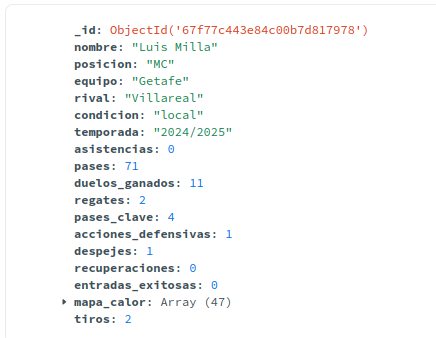
\includegraphics[width=0.7\textwidth]{plantilla-TFG-ETSIIT/doc/imagenes/BD_futbolista.png}
    \caption{Ejemplo almacenamiento de futbolista en BD}
    \label{fig:etiqueta-imagen}
\end{figure}

Para el mapa de calor se almacena como una matriz donde cada entrada tiene 2 coordenadas x e y,  que indican dónde tocó el balón el futbolista dentro del terreno de juego.

\begin{figure}[H]
    \centering
    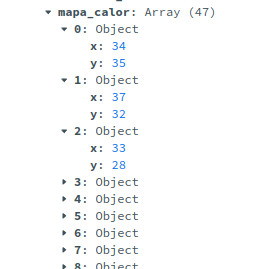
\includegraphics[width=0.7\textwidth]{plantilla-TFG-ETSIIT/doc/imagenes/BD_mapa_calor.png}
    \caption{Ejemplo almacenamiento de mapa de calor en BD}
    \label{fig:etiqueta-imagen}
\end{figure}

Todos los datos empleados en este trabajo han sido obtenidos de la página web de Sofascore \cite{Sofascore}. Cabe señalar que dichos datos están protegidos por derechos de autor y no han sido liberados para su uso público ni académico.

\section{Planteamiento del problema}
El objetivo es desarrollar una expresión analítica basada en sumatorios y ponderaciones que, usando únicamente las estadísticas normalizadas y los mapas de calor, determine el resultado del partido. La idea central es que la aportación de cada equipo se obtenga a partir de la suma de las contribuciones de sus jugadores en distintas zonas del campo, comparándose de forma simétrica las zonas de ataque de un equipo con las zonas defensivas del rival. Para ello, se van a seguir los siguientes pasos:

\begin{enumerate}
    \item \textbf{Separación de las estadísticas por naturaleza ofensiva y defensiva}: Cada jugador posee acciones que favorecen la creacion de juego (constructivas) y acciones que impiden el avance del rival (destructivas). Las acciones consideradas constructivas son: asistencias, tiros, pases, pases clave, regates y duelos ganados. Las acciones defensivas son: acciones defensivas, despejes, recuperaciones, entradas exitosas y paradas.
    \item \textbf{Normalización de las estadísticas}: Todas las estadísticas se normalizan a valores entre 0 y 1, donde 0 indica que la acción no se realizó durante el partido y 1 indica que el jugador fue el máximo ejecutor de esa acción.
    \item \textbf{Impacto espacial a través de heatmaps}: cada jugador tiene un mapa de calor. Se define:
    \begin{itemize}
        \item $ A_i: \text{ área total (número de píxeles) del heatmap del jugador } i.$
        \item $ a_{i,j}: \text{ número de píxeles del jugador } i \text{ que caen en la zona } j. $
        \item $ p_{i,j} = \frac{a_{i,j}}{A_i}; \text{ impacto relativo del jugador } i \text{ en la zona } j. $
    \end{itemize} 

    \item \textbf{División del terreno en zonas:} El campo se divide en un número fijo de 24 zonas asignando a cada una un peso $w_j$ que refleja su importancia. Es importante 
    considerar la simetría ya que la zona que es defensiva para un equipo es ofensiva para el otro (por ejemplo, la portería de uno es el área de ataque del contrario).
    \item \textbf{Predicción del resultado:} A partir de la aportación combinada de todas las zonas y de ambos equipos, se establece un score global que, según su signo (y magnitud),
    predice la victoria del equipo local, la victoria del visitante o un empate.

\end{enumerate}

\section{Desarrollo del modelo matemático}
\subsection*{Separación y normalización de estadísticas}

Cada jugador $i$ registra diversas estadísticas durante el partido, que se dividen en dos
categorías:

\begin{itemize}
    \item \textbf{Juego constructivo (ofensivo):} Conjunto $C$ de acciones que favorecen la creación de juego.
    \item \textbf{Juego destructivo (defensivo):} Conjunto $D$ de acciones que dificultan el avance del rival.
\end{itemize}

Sea $f_{i,k}$ la estadística cruda $k$ del jugador $i$. Para comparar valores entre jugadores y
partidos, cada estadística se normaliza a un valor en el intervalo [0, 1]. Una forma de
normalizar es:
\[
f_{i,k}^{\text{norm}} = \frac{f_{i,k}}{\max\{f_{j,k} : j \text{ en el partido}\}}
\]
donde máx\{$f_{i,k}$\} es el máximo observado de la estadística $k$ en el partido.
Posteriormente, se calculan dos scores diferenciados:
\[
S_i^c = \sum_{k \in C} f_{i,k}^{\text{norm}} \quad y \quad S_i^d = \sum_{k \in D} f_{i,k}^{\text{norm}}
\]

\section{Calculo del impacto espacial mediante el mapa de calor}
Cada jugador dispone de un mapa de calor, que es una representación en píxeles de su
actividad en el terreno durante el partido.
\subsection*{Área total de acción}
Se define el área total de acción del jugador $i$ como:
\[
A_i = \sum_{j=1}^{N} a_{i,j}
\]

donde $a_{i,j}$ es el número de píxeles del heatmap que caen en la zona $j$ y $N$ es el número total de zonas en que se ha dividido el campo, en este caso 24. Esta suma representa la
totalidad de la presencia del jugador en el terreno.

\subsection*{Impacto relativo en cada zona}
Cada zona $j$ del campo se considera una subdivisión del mapa de calor. El impacto o la
proporción de la acción del jugador en la zona $j$ se define como:
\[
p_{i,j} = \frac{a_{i,j}}{A_i}
\]

Este valor indica la fracción del área total de acción del jugador que se concentra en la
zona $j$.

\section{Cáculo de la aportación individual a cada zona}
Se pondera la calidad (score) del jugador por su presencia en cada zona. Así, para
cada jugador $i$ y zona $j$ se definen dos aportaciones:

\begin{itemize}
    \item \textbf{Aportación constructiva:} 
    \[ C^c_{i,j,ofensivo} = p_{i,j} \cdot S_i^c \quad \]
    \item \textbf{Aportación destructiva:}
    \[ \quad C^d_{i,j, defensivo} = p_{i,j} \cdot S_i^d \]
\end{itemize}

De esta forma, se distribuye el desempeño global del jugador en función de la intensidad
de su presencia en distintas áreas del campo.

\section{Aportación total del equipo en cada zona}
Para cada equipo $T$ (local o visitante), se agregan las contribuciones de todos sus
jugadores en cada zona $j$:

\[ C^c_{T,j} = \sum_{i \in T} C^c_{i,j} \quad , \quad C^d_{T,j} = \sum_{i \in T} C^d_{i,j} \]

Esto permite obtener, para cada zona, un indicador global de la capacidad ofensiva y
defensiva del equipo, considerando la distribución espacial de la actividad.

\section{Evaluación de la ventaja zonal y cálculo del score global}
\subsubsection*{Evaluación de las zonas de ataque y defensa}

Para evaluar la ventaja de un equipo se comparan las aportaciones en las zonas correspondientes:

\begin{itemize}
    \item \textbf{Para cada zona del campo} : Se compara la aportación constructiva local con la aportación defensiva del equipo visitante y viceversa:
    \[ \Delta_j = w_{ofensivo} \cdot C^c_{\text{local},j} - w_{defensivo} \cdot C^d_{\text{visitante},m(j)} \]
    
    \[ \Delta_k' = w_{defensivo} \cdot C^c_{\text{visitante},k} - w_{ofensivo} \cdot C^d_{\text{local},m(k)} \]
    
\end{itemize}

Aquí, $w_{ofensivo}$ y $w_{defensivo}$ son los pesos asignados a cada zona, en función de si son estadísticas ofensivas o defensivas (valores en el intervalo [0, 1]) que
reflejan la importancia relativa de cada área del campo.

\subsubsection*{Score global del partido}
Se calcula el score total de cada equipo y se comparan:

\[S_1 = \sum_{j=1}^{N} \Delta_j\] 

\[S_2 = \sum_{k=1}^{N} \Delta_k \]

El score final es la diferencia entre ambos:

\[ S = S_1 - S_2\]

\subsubsection*{Regla de decisión}
La predicción del resultado del partido se basa en el valor de S:
\begin{itemize}
    \item Si $S > \delta$, se predice victoria del equipo local.
    \item Si $S < -\delta$, se predice victoria del visitante.
    \item Si $|S| \leq \delta$, se predice empate.
\end{itemize}

El parámetro $\delta$ es un umbral pequeño que se ajusta para tener en cuenta variaciones o incertidumbres en la estimación; en este caso, se ha decidido, tras varias pruebas hechas a mano, que el valor sea 2.

\section{Algoritmo genético}
En el contexto actual de creciente complejidad en la resolución de problemas computacionales, los algoritmos evolutivos han ganado relevancia como herramientas eficaces para abordar tareas que presentan un elevado grado de dificultad, especialmente aquellas que no pueden resolverse de forma óptima mediante métodos deterministas tradicionales. Entre estos algoritmos, los algoritmos genéticos destacan por su capacidad para encontrar soluciones aproximadas de alta calidad en espacios de búsqueda amplios.

Inspirados en los principios de la evolución natural propuestos por Charles Darwin, los algoritmos genéticos simulan procesos como la selección natural, el cruce genético y la mutación para evolucionar una población de posibles soluciones hacia un óptimo. Gracias a su carácter exploratorio y adaptativo, los algoritmos genéticos han sido aplicados con éxito en diversas áreas, como la optimización de funciones, el diseño de redes neuronales, la planificación de rutas o la programación automática.

El objetivo del algoritmo genético aplicado a mi proyecto es tratar de encontrar unos vectores de pesos de ataque y defensa adecuados para ponderar las distintas zonas del campo, ya que hasta ahora se habían elegido de manera manual, aunque con cierta lógica.

Para implementarlo, los individuos de la población estarían formados por los vectores de ataque y defensa unidos en uno solo, y el objetivo sería maximizar según la función de evaluación que se basa en ejecutar el vector en todos los partidos de la base de datos, dando un porcentaje de acierto del vector. Para ello se utilizan distintos atributos de población, tasa de mutación y número de generaciones, y se prueban las combinaciones de todos para quedarnos con la mejor. Las especificaciones de los atributos y su implementación se pueden ver en la sección 5.4, Algoritmo genético.


\subsection*{Otros algoritmos}
Se ha implementado también el mismo algoritmo genético, pero con $\delta$, es decir, se puede predecir el vector de pesos y $\delta$, que es el valor que permite definir a partir de dónde se decide el ganador del partido, que hasta ahora había sido puesto a 2 de manera manual. Las especificaciones de los atributos y su implementación se pueden ver en la sección 5.5, Algoritmo genético con $\delta$.

Por último, se ha implementado un algoritmo donde no se tiene en cuenta el mapa de calor de los futbolistas con el objetivo de mostrar la comparación de los resultados cuando estos no se usan.
Su implementación se puede consultar en la sección 5.2, Algoritmo sin pesos,


